\section{Introduction}

As has been pointed out by the incident at the Ketelbrug between Emmeloord and Lelystad, bridges require a watertight control system.  Many examples exist where bridges are not opened or closed properly, bridge components break down or the bridge is being stuck in a particular state. The goal of this project is to design a safety layer that can be added to the main control interface, in order to capture all possible situations and failures.

In order to achieve this, we first define all requirements that must be met by the bridge. This is being done both informally and formally using $\mu$-calculus, a modal logic in which properties can be expressed. Then, we model the bridge using mCRL2\footnote{mCRL2 toolset 201310.0}, a tool to create concurrent discrete event systems. Within this program, the $\mu$-calculus requirements can be verified. This step will result in a verification overview of all the requirements of our bridge. After this, we will make the model open to user input by verifying the safety for all actions in each state. By doing this, the system also covers the realistic event of the bridge operator interrupting the system.

Modeling the bridge can be done in various levels of detail. For our model, we make use of the following assumptions:
%
\begin{itemize}
	\item When a bridge component is to be said in a particular state, this implies that the majority of the sensors have detected the bridge to be in this state (e.g. if the bridge is considered open, three or four sensors have detected the bridge deck to be open.)
	\item	The individual sensors of the components (sign, barrier or lock) communicate with the control system by means of one signal (so they always agree on the bridge status)
	\item If a communication has been established between two regarding the status, it means that a \texttt{send} action from component A has been received, processed and confirmed by object B
	\item If a communication has been established between two components regarding an action, it means that a \texttt{send} action from object A has been received, processed and executed by object B
	\item In order for a required to be satisfied, it must be satisfied for all instances of the components (e.g. \emph{all} pre signs must be switched on in order for a stop sign to be switched on)
\end{itemize}
%
In the next subsection, the desired behaviour of the bridge is being determined and defined. Section \ref{sec:glob} contains the global requirements that will be met in our system. Specific interactions that can be performed by the bridge are discussed in Section \ref{sec:act}, whereas section \ref{sec:arch} discusses the used architecture of the system. In section \ref{sec:trans} the requirements stated earlier are translated into these interactions. The modeling of the bridge is covered by section \ref{sec:model}, followed by section \ref{sec:check} holding the results of the system validation. Finally, the conclusion can be found in section \ref{sec:conclusion}.

\subsection{Desired behavior of the bridge}

Although it seems pretty straightforward what should be the desired behavior of a bridge, the Ketelbrug accident shows us that this can be slightly more complicated than it appears. For the project, the Project Guide\footnote{J. J. A. Keiren, System Validation (IN4387) Project Guide, VU University Amterdam, november 2013} has described the desired behavior in detail. For the sake of the clarity of this report, the general outline is repeated here. The bridge has two main modes: open and close. Sequences \ref{tab:open} and \ref{tab:close} below shows all steps that need to be taken to open and close the bridge.
%
\begin{table}[h]%
\begin{tabular}{l}
	\footnotesize
	\texttt{switch on pre signs -> switch on stop signs -> lower barriers -> disengage locks -> lift bridge deck}\\
\end{tabular}
\caption{Steps to be taken when opening the bridge.}
\label{tab:open}
\end{table}
%
\begin{table}[h]%
\begin{tabular}{l}
	\footnotesize
	\texttt{lower bridge deck -> engage locks -> raise barriers -> switch off stop signs -> switch off pre signs}\\
\end{tabular}
\caption{Steps to be taken when closing the bridge.}
\label{tab:close}
\end{table}
%
The most important feature is that every action can only be performed when the previous action has already occurred properly (according to assumptions we stated earlier). For example, it undesireable for cars to have a barrier coming down when no warning sign has been switched on previously. Also, the system has to be free of deadlocks. 

In the following sections of the report, the bridge components will be labelled with individual identifiers. These are based on figure \ref{fig:setup}, an image from the project guide. 
%
\begin{figure}[htb]%
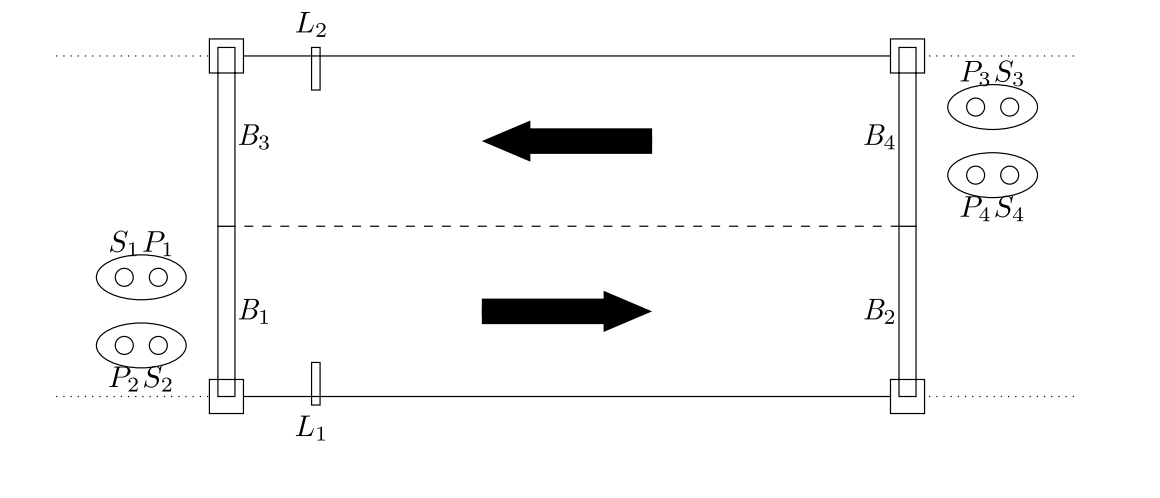
\includegraphics[width=\columnwidth]{Images/Setup.png}%
\caption{Setup of the bridge, using labelled components (from: Project Guide)}%
\label{fig:setup}%
\end{figure}
%

\newpage